%%%%%%%%%%%%%%%%%%%%%%%%%%%%%%%%%%%%%%%%%
% Programming/Coding Assignment
% LaTeX Template
%
% This template has been downloaded from:
% http://www.latextemplates.com
%
% Original author:
% Ted Pavlic (http://www.tedpavlic.com)
%
% Note:
% The \lipsum[#] commands throughout this template generate dummy text
% to fill the template out. These commands should all be removed when 
% writing assignment content.
%
% This template uses a Perl script as an example snippet of code, most other
% languages are also usable. Configure them in the "CODE INCLUSION 
% CONFIGURATION" section.
%
%%%%%%%%%%%%%%%%%%%%%%%%%%%%%%%%%%%%%%%%%

%----------------------------------------------------------------------------------------
%	PACKAGES AND OTHER DOCUMENT CONFIGURATIONS
%----------------------------------------------------------------------------------------

\documentclass[a4paper]{article}

\usepackage{fancyhdr} % Required for custom headers
\usepackage{lastpage} % Required to determine the last page for the footer
\usepackage{extramarks} % Required for headers and footers
\usepackage[usenames,dvipsnames]{color} % Required for custom colors
\usepackage{graphicx} % Required to insert images
\usepackage{listings} % Required for insertion of code
\renewcommand*{\lstlistingname}{代码} % change "Listing <ref> to 代码 <ref>
\usepackage{courier} % Required for the courier font
\usepackage{lipsum} % Used for inserting dummy 'Lorem ipsum' text into the template

\usepackage[UTF8]{ctex} % Required for Chinese character
\usepackage{tocloft} % Required for beautiful toc
\usepackage[hidelinks]{hyperref} % Required for clickable toc
\hypersetup{
    colorlinks,
    citecolor=black,
    filecolor=black,
    linkcolor=black,
    urlcolor=black
}
\usepackage[title]{appendix} % Required for appendix

% Margins
\topmargin=-0.45in
\evensidemargin=0in
\oddsidemargin=0in
\textwidth=6.5in
\textheight=9.0in
\headsep=0.25in

\linespread{1.1} % Line spacing

% Set up the header and footer
\pagestyle{fancy}
\lhead{\hmwkAuthorName} % Top left header
\chead{\hmwkClass\ (\hmwkClassInstructor\ \hmwkClassTime): \hmwkTitle} % Top center head
\rhead{\firstxmark} % Top right header
\lfoot{\lastxmark} % Bottom left footer
\cfoot{} % Bottom center footer
\rfoot{Page\ \thepage\ of\ \protect\pageref{LastPage}} % Bottom right footer
\renewcommand\headrulewidth{0.4pt} % Size of the header rule
\renewcommand\footrulewidth{0.4pt} % Size of the footer rule

\setlength\parindent{0pt} % Removes all indentation from paragraphs

%----------------------------------------------------------------------------------------
%	CODE INCLUSION CONFIGURATION
%----------------------------------------------------------------------------------------

\definecolor{MyDarkGreen}{rgb}{0.0,0.4,0.0} % This is the color used for comments
\lstloadlanguages{Perl} % Load Perl syntax for listings, for a list of other languages supported see: ftp://ftp.tex.ac.uk/tex-archive/macros/latex/contrib/listings/listings.pdf
\lstset{language=Perl, % Use Perl in this example
        frame=single, % Single frame around code
        basicstyle=\small\ttfamily, % Use small true type font
        keywordstyle=[1]\color{Blue}\bf, % Perl functions bold and blue
        keywordstyle=[2]\color{Purple}, % Perl function arguments purple
        keywordstyle=[3]\color{Blue}\underbar, % Custom functions underlined and blue
        identifierstyle=, % Nothing special about identifiers                                         
        commentstyle=\usefont{T1}{pcr}{m}{sl}\color{MyDarkGreen}\small, % Comments small dark green courier font
        stringstyle=\color{Purple}, % Strings are purple
        showstringspaces=false, % Don't put marks in string spaces
        tabsize=5, % 5 spaces per tab
        %
        % Put standard Perl functions not included in the default language here
        morekeywords={rand},
        %
        % Put Perl function parameters here
        morekeywords=[2]{on, off, interp},
        %
        % Put user defined functions here
        morekeywords=[3]{test},
       	%
        morecomment=[l][\color{Blue}]{...}, % Line continuation (...) like blue comment
        numbers=left, % Line numbers on left
        firstnumber=1, % Line numbers start with line 1
        numberstyle=\tiny\color{Blue}, % Line numbers are blue and small
        stepnumber=2, % Line numbers go in steps of 5,
        firstnumber=1
}

% Creates a new command to include a perl script, the first parameter is the filename of the script (without .pl), the second parameter is the caption
\newcommand{\perlscript}[2]{
\begin{itemize}
\item[]\lstinputlisting[caption=#2,label=#1]{#1.pl}
\end{itemize}
}

\newcommand{\shfilescript}[3]{
\begin{itemize}
\item[]\lstinputlisting[caption=#2, label=#1, language=sh]{#3}
\end{itemize}
}
\newcommand{\shscript}[3]{
\begin{itemize}
\item[]\begin{lstlisting}[label=#1, caption=#2] #3 \end{lstlisting}
\end{itemize}
}

%----------------------------------------------------------------------------------------
%	DOCUMENT STRUCTURE COMMANDS
%	Skip this unless you know what you're doing
%----------------------------------------------------------------------------------------

% Header and footer for when a page split occurs within a problem environment
\newcommand{\enterProblemHeader}[1]{
\nobreak\extramarks{#1}{#1 见下页\ldots}\nobreak{} 
\nobreak\extramarks{接上页}{#1 见下页\ldots}\nobreak{}
}

% Header and footer for when a page split occurs between problem environments
\newcommand{\exitProblemHeader}[1]{
\nobreak\extramarks{接上页}{#1 见下页\ldots}\nobreak{}
\nobreak\extramarks{#1}{}\nobreak{}
}
% TODO:code here enable the number before section, but it disable the numbering of problems
%\setcounter{secnumdepth}{0} % Removes default section numbers
\newcounter{homeworkProblemCounter} % Creates a counter to keep track of the number of problems

\newcommand{\homeworkProblemName}{}

\newenvironment{homeworkProblem}[1][Problem \arabic{homeworkProblemCounter}]{ % Makes a new environment called homeworkProblem which takes 1 argument (custom name) but the default is "Problem #"
\stepcounter{homeworkProblemCounter} % Increase counter for number of problems
\renewcommand{\homeworkProblemName}{#1} % Assign \homeworkProblemName the name of the problem
\section{\homeworkProblemName} % Make a section in the document with the custom problem count
\enterProblemHeader{\homeworkProblemName} % Header and footer within the environment
}{
\exitProblemHeader{\homeworkProblemName} % Header and footer after the environment
}

\newcommand{\problemAnswer}[1]{ % Defines the problem answer command with the content as the only argument
\noindent\framebox[\columnwidth][c]{\begin{minipage}{0.98\columnwidth}#1\end{minipage}} % Makes the box around the problem answer and puts the content inside
}

\newcommand{\homeworkSectionName}{}
\newenvironment{homeworkSection}[1]{ % New environment for sections within homework problems, takes 1 argument - the name of the section
\renewcommand{\homeworkSectionName}{#1} % Assign \homeworkSectionName to the name of the section from the environment argument
\subsection{\homeworkSectionName} % Make a subsection with the custom name of the subsection
\enterProblemHeader{\homeworkProblemName\ [\homeworkSectionName]} % Header and footer within the environment
}{
\enterProblemHeader{\homeworkProblemName} % Header and footer after the environment
}


\newcommand{\codev}[1]{\textsf{#1}}
%----------------------------------------------------------------------------------------
%	NAME AND CLASS SECTION
%----------------------------------------------------------------------------------------

\newcommand{\hmwkTitle}{操作系统原理实验\ \#1} % Assignment title
\newcommand{\hmwkDueDate}{Monday,\ March\ 12,\ 2018} % Due date
\newcommand{\hmwkClass}{16级计科\ 7班} % Course/class
\newcommand{\hmwkClassTime}{周一9-10节} % Class/lecture time
\newcommand{\hmwkClassInstructor}{凌应标} % Teacher/lecturer
\newcommand{\hmwkAuthorName}{颜彬} % Your name
\newcommand{\hmwkAuthorId}{16337269} % Your id 

%----------------------------------------------------------------------------------------
%	TITLE PAGE
%----------------------------------------------------------------------------------------

\usepackage{titling}

\title{
\vspace{2in}
\textmd{\textbf{\hmwkClass:\ \hmwkTitle}}\\
\normalsize\vspace{0.1in}\small{Due\ on\ \hmwkDueDate}\\
\vspace{0.1in}\large{\textit{\hmwkClassInstructor\ \hmwkClassTime}}
\vspace{3in}
}

\author{\textbf{\LARGE{\hmwkAuthorName}} \\ \\ \textbf{\LARGE{\hmwkAuthorId}}}
\date{} % Insert date here if you want it to appear below your name
%----------------------------------------------------------------------------------------

\begin{document}
% \begin{titlingpage} % This is for ignore page number in first page. package titling

\maketitle

%----------------------------------------------------------------------------------------
%	TABLE OF CONTENTS
%----------------------------------------------------------------------------------------

\setcounter{tocdepth}{2} % Uncomment this line if you don't want subsections listed in the ToC


\renewcommand{\cftsecleader}{\cftdotfill{\cftdotsep}} % used for dots between <section> and <page>
\renewcommand{\contentsname}{Content} % force the word to be "content
\newpage
\tableofcontents
\addtocontents{toc}{~\hfill\textbf{Page}\par}
\newpage

% below are document body


% To have just one problem per page, simply put a \clearpage after each problem
\section{实验目的}
掌握操作系统的相关概念,理解计算机引导的全部过程。利用工具制作正确引导盘并完成特定任务。\\ 

理解虚拟机的运行方式,了解虚拟机与真实机器的不同之处。熟悉配置、运行虚拟机的基本方法。掌握在虚拟机下运行程序、程序
查错和运行dos镜像。\\ 

熟悉相关工具的使用。熟悉32位x86汇编器和二进制文件操作软件的使用。熟悉虚拟镜像的制作方法。
掌握基本的32位x86汇编的编写。掌握汇编程序的编译、运行、调错。掌握硬件级的调试技巧。
\section{实验要求}

\subsection{搭建和应用实验环境}
虚拟机安装,生成一个基本配置的虚拟机 XXXPC 和多个 1.44MB 
容量的虚拟软盘,将其中一个虚拟软盘用 DOS 格式化为 DOS 引导盘,用 WinHex 工具将其中一个虚拟软盘的首扇区填满你的个人信息。
\subsection{接管裸机控制权}
设计 ibmpc 的一个引导扇区程序
,程序功能从屏幕左边某行位置45度
角斜向下射出,保持一个可观察的适当速度直线运动,在碰到屏幕边后产生反射,
改变方向运动,如此类推,不断运动。在此基础上,增加你的个性拓展,如同时控制两个运动的轨迹,
或炫酷动态变色,个性画面,如此等等,自由不限。还要在屏幕某个区域以特别的方式显示你的学号姓名
等个人信息。将这个程序的机器吗放到第三张虚拟软盘的首扇区,并用此软盘引导你的pc,直到成功。


\section{实验方案}
\subsection{基础原理}
实验环境是不带有操作系统的裸机。为了做到接管逻辑控制权和运行程序的目的,我们需要写出自己的引导程序(制作一个引导扇区)。
开机后,计算机会首先作自检。若选择从软盘启动,bios会检查软盘的0面0磁道1扇区,如果发现它的最后一个字节是0xAA55,则bios会把其视作一个引导扇区,
尝试执行其中的程序。\\ 

引导扇区通常会将操作系统加载进内存中,将控制权完全交给操作系统,由操作系统完成随后的各种调配。在本实验中,引导扇区内包含了
若干代码,用于在屏幕中心高亮显示个人信息,以及完成简单的动画。 \\

即便没有操作系统,本次实验依然可以在终端输出相应的信息,甚至是绘制动画。
0xB8000-0xBFFFF的内存空间是显存地址,共有32KB。向这个地址写入数据可以打印到屏幕上。
对于从0xB800开始的每个字\(16 bits\),其高位将解释为输出内容的样式信息,例如前景色、背景色等;其低位将解释为输出内容的Ascii码。\\

通过反复往显存地址中读写数据,本项目最终完成了附带个人资料和动画的引导程序。



\subsection{实验环境与工具}
\subsubsection{实验环境}
\begin{itemize}
    \item 操作系统 \\ 
    本实验在Linux下完成。采用Ubuntu 16.04
    \item 虚拟机\\
    bochs.它是一款开源且跨平台的 IA-32 模拟器。
\end{itemize}
\subsubsection{相关工具、指令}
\begin{itemize}
    \item 汇编器\\ 
    NASM. NASM是一个轻量级的、模块化的 80x86 和 x86-64 汇编器。它的语法与
    Intel 原语法十分相似,但更加简洁和易读。它对宏有十分强大的支持。
    \item 镜像文件产生工具\\ 
    bximage. 该命令允许生成指定大小的软件镜像。
    \item 二进制写入命令\\ 
    dd. dd 允许指定源文件和目标文件,将源文件的二进制比特写入目标文件中的指定位置。
    \item 二进制文件查看命令\\ 
    xxd. xxd 允许将二进制文件中的内容按地址顺序依次输出,可读性强
\end{itemize}
关于工具dd和xxd的使用,请见附录\ref{utilitycode}代码\ref{buildFile}
\subsection{程序流程}\label{programProcedure}
图\ref{fig:procedure}展示了程序stone.asm的流程图。\\

其中"设定延时"步骤将初始化一个循环。该循环不断检测某个变量\codev{count}是否已经达到特定的值。若未达到,则将\codev{count}加1,
继续执行下一个循环。若\codev{count}达到了预设的值,则跳出循环,继续执行下面的语句(相当于执行一个\codev{callback function})。
当\codev{callback}的语句执行完毕后,末尾的\codev{jmp}指令将把程序再次带入延时循环。
\begin{figure}  
    \begin{center}  
    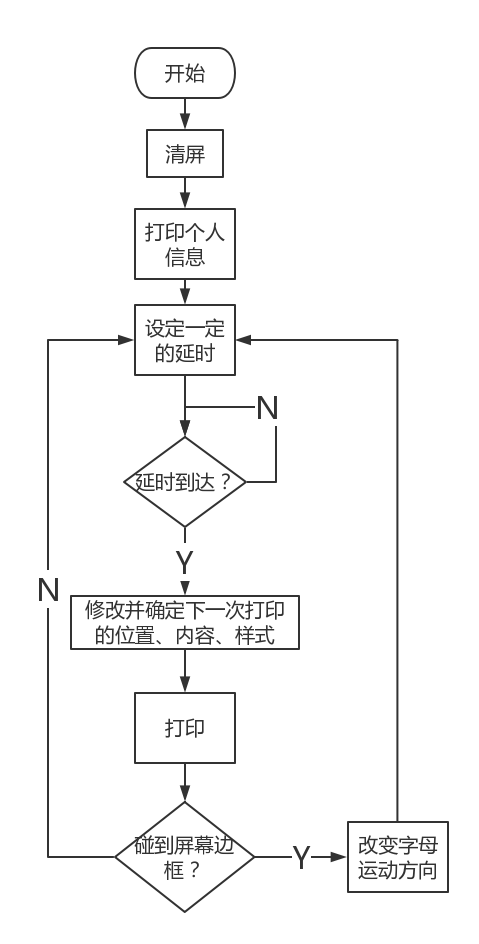
\includegraphics[scale=0.5]{asset/procedure.png}  
    \caption{stone.asm流程图.\label{fig:procedure}}  
    \end{center}  
\end{figure}  

\subsection{程序模块及相关说明}\label{modelIntroduction}
\subsubsection{实现引导}
如代码\ref{boot}所示,在程序的末尾加上该代码片段。\\

其中\$代表当前行的地址。\$\$代表当前扇区的首地址。所以510-(\$-\$\$)代表当前行距离扇区末尾的长度再减二字节。
减二字节是为了在扇区的最后预留空间给0xAA55,以使得系统识别该盘为引导盘。
\begin{figure}
\begin{itemize}
\item[] \begin{lstlisting}[language={[x86masm]Assembler}, label=boot, caption=使软盘成为引导盘的关键代码]
    ; ...
    times 510-($-$$) db 0
    dw 0xaa55
\end{lstlisting}
\end{itemize}
\end{figure}
\subsubsection{延时循环}

代码\ref{delay}展示了延时循环的相关代码。\\

在延时循环中,代码会不断地将
50000 * 580 这一值减一。当这一值减
为0时,执行后面的\codev{main:}标签部分,达到延时的效果。
值得注意的是,50000 * 580 这一值较大,无法直接存入一个32位变量中,故程序采用
\codev{word[count]} 和 \codev{word[dcount]} 两个变量的乘法表示这一整数。\\

\begin{figure}
\begin{itemize}
\item[] \begin{lstlisting}[language={[x86masm]Assembler}, label=delay, caption=延时循环]
loop1:
    dec word[count]		
    jnz loop1			
    mov word[count],delay
    dec word[dcount]			
    jnz loop1
    mov word[count],delay
    mov word[dcount],ddelay
main:
    ; code below ...
\end{lstlisting}
\end{itemize}
\end{figure}
\subsubsection{清屏模块}
代码\ref{clearScreen}展示了清屏模块的主要内容。\\ 

在清屏模块中,程序首先计算出屏幕大小\codev{ScreenLength}(单位字节)。随后进入一个循环
,在循环内部反复将0xB800随后的\codev{ScreenLength}长度的内存区域置为0,达到清屏效果。\\

代码中,\codev{gs}指向显存段地址,即0xB800.\codev{cx}为计数器,在\codev{loop}中
逐次-1.
\begin{figure}
\begin{itemize}
\item[] \begin{lstlisting}[language={[x86masm]Assembler}, label=clearScreen, caption=清屏模块]
ScreenLength equ 80 * 25 * 2
; ...
clearTheScreen:
    mov cx, ScreenLength
    mov bx, 0
clearScreenLoop:
    loop clearWorker
    ret
clearWorker:
    mov word[gs:bx], 0
    inc bx
    jmp clearScreenLoop
\end{lstlisting}
\end{itemize}
\end{figure}

\subsubsection{修改显存区}
代码\ref{show}展示了用于修改显存的代码片段。\\

显示模块的重点在于计算数据的显示位置,以及将数据写入正确的内存地址中\\

由于屏幕为25行80列,所以对于x行y列的数据而言,其索引应为\codev{80x + y}.由于显存采用字长作为显示
单元,故该数据应该写入的内存地址为"显存段首地址:\codev{2*(80x + y)}"。
在整个程序中,\codev{gs}已被初始化为显存段地址0xB800,故\codev{[gs:bx]}将
指向写入的内存地址。\\

代码\ref{show}省略了部分细枝末节的部分。代码假定ax中存储了打印的
有关信息,其中高位\codev{ah}存储了打印的样式,例如前景色和背景色等;
低位\codev{al}存储了打印的字符对应的ASCII码。
\begin{figure}
\begin{itemize}
\item[] \begin{lstlisting}[language={[x86masm]Assembler}, label=show, caption=show模块]
show:
    ; ...
    xor ax,ax ; set ax to 0            
    mov ax,word[x]
    mov bx,80
    mul bx
    add ax,word[y] ; ax = 80 * x + y
    mov bx,2
    mul bx
    mov bx,ax ; bx = 2(80 * x + y)
    ; ...
    mov [gs:bx],ax 
    ret
\end{lstlisting}
\end{itemize}
\end{figure}
\section{实验过程}
\subsection{用Dos制作引导盘}
首先需要创建一个虚拟软盘。如代码\ref{createImg}所示,在linux下采用bximage命令,产生一个1.44Mb,命名为\codev{a.img}的虚拟镜像。
本实验采用bochs虚拟机,故首先需要在bochs官网下下载FreeDos镜像。镜像下载完毕后,解压,将其中的
\codev{a.img}文件重命名为\codev{freedos.img}。\\

bochs默认采用\codev{.bochsrc}文件为配置文件。按照代码\ref{config}的方式配置bochs,
使其以freedos.img为A盘,以空镜像a.img为B盘,并设置A盘为启动盘。\\

随后,如代码\ref{createImg}后半部分所示,运行bochs,进入dos系统,格式化B盘。此时B盘即成为引导盘。

\begin{figure}
\begin{itemize}
\item[] \begin{lstlisting}[language=sh, label=createImg, caption=创建虚拟软盘]
$ bximage
    // ... ignore outputs

$ bochs
...format B:
\end{lstlisting}
\end{itemize}
\end{figure}

\begin{figure}
\begin{itemize}
\item[] \begin{lstlisting}[label=config, caption=.bochsrc文件部分节选]
...
floppya: 1_44=freedos.img, status=inserted
floppyb: 1_44=a.img, status=inserted

boot: a
...
\end{lstlisting}
\end{itemize}
\end{figure}
\subsection{扇区填充个人信息}
本问题采用更灵活的方式实现。\\

如代码\ref{personal}所示,利用nasm的语法特性,产生数个个人信息的字符串,用于填满软盘空间。
随后,如代码\ref{genPersonal}所示,直接将编译后的所有二进制信息写入\codev{fill.img}中。此时\codev{fill.img}
内即填满了所有的个人信息。
\begin{figure}
\begin{itemize}
    \item[] \lstinputlisting[language={[x86masm]Assembler}, label=personal, caption=来自fill.asm文件内容]{../../section2/fill.asm}
\end{itemize}
\end{figure}

\begin{figure}
\begin{itemize}
\item[] \begin{lstlisting}[language=sh, label=genPersonal, caption=编译fill.asm并将内容写入fill.img]
$ nasm fill.asm -o fill.bin 
$ dd if=fill.bin of=fill.img
\end{lstlisting}
\end{itemize}
\end{figure}

\subsection{接管裸机的控制权}
如\ref{modelIntroduction}节和\ref{programProcedure}所示,按照该思路实现
\codev{stone.asm}文件,并采用\ref{complile}节所示的方法编译,\ref{sec:run}节所示的方法
运行代码。结果见\ref{result}节。

\section{实验结果}
    \subsection{代码编译(可选)}\label{complile}
    在项目文件中已经包括了产生的所有代码。所以这一步可以跳过\\ 
    代码 \ref{build}展示了将汇编最终写入镜像文件的方法。
    它将首先使用nasm将.asm文件编译为.bin文件。随后使用dd将.bin的内容写入.img中。

    \begin{itemize}
    \item[] \begin{lstlisting}[language=sh, label=build, caption=将汇编转化为二进制并写入镜像]
    $ bximage # 先用该命令产生空白的stone.img文件
    $ sh build.sh
    \end{lstlisting}
    \end{itemize}
    代码\ref{build}的内容请见附录\ref{utilitycode}的代码\ref{buildFile}


    \subsection{运行代码}\label{sec:run}
    按代码\ref{run}的方式运行脚本,即可运行\codev{stone.asm}程序。
    在这一步中,脚本会调用bochs运行完成好的镜像文件。bochs将自动加载相同目录内的
    \codev{.bochsrc}文件,以此为配置运行虚拟机。
    \begin{itemize}
        \item[] \begin{lstlisting}[label=run, caption=运行方法]
$ sh run.sh
        \end{lstlisting}
    \end{itemize}
    
    代码\ref{run}的内容见附录\ref{utilitycode}代码\ref{runFile}

    \subsection{结果展示}\label{result}
    \subsubsection{Dos制作的启动盘}
    代码\ref{dosBoot}列出了由dos格式化后得到的启动盘的具体信息。
    \begin{figure}
    \begin{itemize}
    \item[] \begin{lstlisting}[label=dosBoot, caption=Dos下制作的引导盘a.img的部分内容]
        00000000: eb3c 9046 7265 6544 4f53 0000 0201 0100  .<.FreeDOS......
        00000010: 02e0 0040 0bf0 0900 1200 0200 0000 0000  ...@............
        00000020: 0000 0000 0100 2900 0000 0020 2020 2020  ......)....
        00000030: 2020 2020 2020 4641 5431 3220 2020 0e1f        FAT12   ..
        00000040: be5b 7cac 22c0 740b 56b4 0ebb 0700 cd10  .[|.".t.V.......
        00000040: be5b 7cac 22c0 740b 56b4 0ebb 0700 cd10  .[|.".t.V.......
        00000050: 5eeb f032 e4cd 16cd 19eb fe54 6869 7320  ^..2.......This
        00000060: 6973 206e 6f74 2061 2062 6f6f 7461 626c  is not a bootabl
        00000070: 6520 6469 736b 2e20 2050 6c65 6173 6520  e disk.  Please
        00000080: 696e 7365 7274 2061 2062 6f6f 7461 626c  insert a bootabl
        00000090: 6520 666c 6f70 7079 2061 6e64 0d0a 7072  e floppy and..pr
        000000a0: 6573 7320 616e 7920 6b65 7920 746f 2074  ess any key to t
        000000b0: 7279 2061 6761 696e 202e 2e2e 200d 0a00  ry again ... ...
        ......
        000001f0: 0000 0000 0000 0000 0000 0000 0000 55aa  ..............U.
    \end{lstlisting}
    \end{itemize}
    \end{figure}

    \subsubsection{写满个人信息的虚拟软盘}
    代码\ref{imagePersonal}展示了文件fill.img的部分情况。\\
    
    \begin{figure}
    \begin{itemize}
    \item[] \begin{lstlisting}[label=imagePersonal, caption=节选自fill.img]
        00000000: 3136 3333 3732 3639 2079 616e 6269 6e20  16337269 yanbin
        00000010: 3136 3333 3732 3639 2079 616e 6269 6e20  16337269 yanbin
        ......
        000001e0: 3136 3333 3732 3639 2079 616e 6269 6e20  16337269 yanbin
        000001f0: 3136 3333 3732 3639 2079 616e 6269 6e20  16337269 yanbin
    \end{lstlisting}
    \end{itemize}
    \end{figure}
    
    \subsubsection{引导程序运行状况}
    图片\ref{fig:stone_run}展示了在bochs下运行stone.asm机器码的实际图片。其中图中心的个人信息会不断闪烁高亮。\\
    
    \begin{figure}
        \begin{center}
        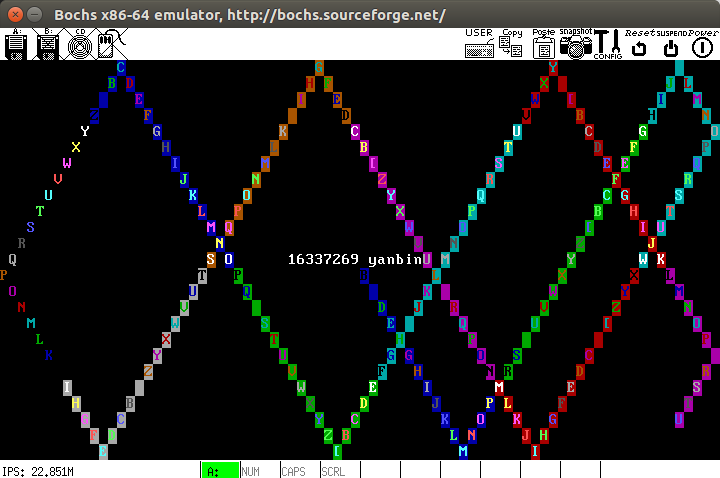
\includegraphics[scale=0.45]{asset/stone_run.png}
        \caption{stone.asm在bochs下的运行截图\label{fig:stone_run} }
        \end{center} 
    \end{figure} 
    
\section{实验总结}
\subsection{心得体会}
这次实验,从配置环境开始,就是对我自己的一大挑战。\\ 

在阅读了《ORANGE’S:一个操作系统的实现.于渊》的前两章后,我发现它的内容与
本次实验比较契合。于是我就萌生了按照这本书的方式配置和实现本项目的想法。由于我
常年用Linux系统,所以从最开始,我便一直考虑着在Linux下完成操作系统的所有项目。这刚好
又于上书是契合的。上书也主要采用Linux系统作为讲解。\\ 

选择了Linux,一方面意味着众多极其强大的开源软件,另一方面也意味着,我将走和许多同学
不同的道路,用几乎完全不同的工具链。毕竟老师给出的工具包的内容几乎是Windos下的开发工具。
我其实并不担心工具的问题,因为使用Linux的经验告诉
我,Linux的组件往往比Windows更丰富,配置也更简单,摸索出属于自己的工具链并不是一件难事。
我最担心的问题是,身边的同学如果大部分使用Windows来开发,那么我在Linux下遇到问题将
很难找到讨论的伙伴。所幸,我的朋友王永锋同学也选择Linux下开发,于是这敲定了我所使用的
环境,并让我配置出了自己较为舒适的工具链。nasm编译,bochs作为虚拟机运行程序和调试程序。
dd, bximage, xxd命令予以协助。\\

令人感到不适的是,网上关于nasm和bochs的相关讨论非常少。在stackoverflow上几乎搜不到
我遇到的关于nasm的讨论。但好在nasm的官方文档写得比较用心,而且我个人的英语也不差,于是
把文档的前几章大概看完了。看完的同时我也体会到nasm比别的汇编器更强大的地方。可以说
官方文档几乎成为了我学习、查询nasm语法的唯一方法。\\

对程序的debug也是这个项目的一大挑战。刚好bochs自带调试功能,这给我带来了很大的便利。
bochs在google上也几乎没有第三方的tutorial,我也只好把bochs的debug文档通读了一遍。
bochs几乎具有我所期望的debugger的所有需求,唯一让我失望的是它的反汇编功能
(个人认为)还不够强大。如果我想要把汇编文档的语句对应到bochs调试时执行的语句,我
需要指定语句的内存地址。然而在实际调试中,确定内存地址是一件很繁琐的事情。但在其他方面
bochs都足够让我调试程序了。与上古程序员相比,我们的工具其实已经很丰富了。\\ 

本次实验,我的收获十分巨大。在上这门课之前,我对操作系统几乎一无所知。对我而言
操作系统就如一个黑箱,我仅仅知道它是一个程序,它负责调配资源,并把极其复杂的硬件
底层信息隔离在程序员的视线之外。在经过这个实验之后,最起码我已经明白了操作系统
最初是如何进入到内存中的。\\

这个实验给我带来的成就感最大的地方在于,我独立地制作出了引导盘,并在上面运行了我
的DIY程序。在实验开始前,我十分惧怕与硬件打交道,害怕硬件中繁复的细节。但在我的最简单
的引导正确输出了“helloworld”之后,我意识到,硬件也并没有我想的那么复杂。硬件
有它自己的规定,按照硬件的规定实现代码,我们依旧可以完全地控制硬件,让它为我们所用。\\ 

凌老师曾有过一个比喻,这个实验“就像一个种子,它落到土里会生根发芽”。虽然这个引导程序
几乎没有干十分特别的事,但它是独立运行在裸机上的。这就意味着,这个引导程序将成为
我们实现操作系统的根基。以后实验的所有代码会直接依赖于这一段程序。。

希望我能在以后的实验中,对操作系统的各种概念理解得更加深刻,逐步完成好属于我自己的操作系统。
\subsection{遇到的BUG}
\subsubsection{MUL指令}
16位和32位的MUL指令会将高位的进位置于dx/edx寄存器中。我一开始并没有留意到这个情况
只是发现dx寄存器会被莫名其妙地清零。现象可复现。\\

发现这个bug并解决的方法是使用bochs调试。我先找到``因为dx清零而出错”的地方,在这个地方设置断点,
单步执行并输出所有的寄存器的值。最终发现在MUL指令的前后dx的值发生了变化。通过参考wikibook的解释,
我理解了bug的原因,并修改了代码
\begin{appendices}
\section{参考文献}
\label{reference}
\begin{enumerate}
    \item http://www.nasm.us/doc/ \\
    for nasm
    \item https://en.wikibooks.org/wiki/X86\_Assembly \\
    for 32bit x86
  \end{enumerate}
    \section{辅助代码}\label{utilitycode}
    \shfilescript{buildFile}{build.sh文件内容}{../build.sh}
    \shfilescript{runFile}{run.sh文件内容}{../run.sh}
    \begin{itemize}
        \item[]\lstinputlisting[label=configAll, caption=.bochsrc文件,作为bochs的配置文件以运行stone.asm]{../.bochsrc}
    \end{itemize}
\end{appendices}
\end{document}